


\tikzset{every picture/.style={line width=0.75pt}} %set default line width to 0.75pt        

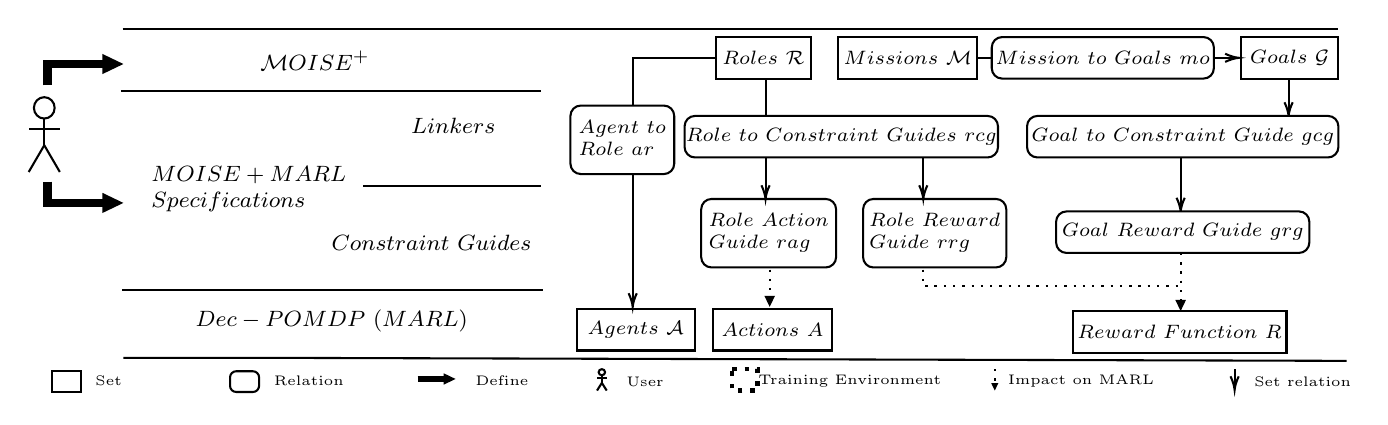
\begin{tikzpicture}[x=0.75pt,y=0.75pt,yscale=-1,xscale=1]
%uncomment if require: \path (0,2584); %set diagram left start at 0, and has height of 2584

%Straight Lines [id:da7190867244927197] 
\draw    (53.43,1976.58) -- (256,1976.58) ;
%Straight Lines [id:da5752020148648518] 
\draw    (466,1960.58) -- (528,1960.58) -- (590,1960.58) ;
\draw [shift={(592,1960.58)}, rotate = 180] [color={rgb, 255:red, 0; green, 0; blue, 0 }  ][line width=0.75]    (6.56,-1.97) .. controls (4.17,-0.84) and (1.99,-0.18) .. (0,0) .. controls (1.99,0.18) and (4.17,0.84) .. (6.56,1.97)   ;
%Straight Lines [id:da4718294533079477] 
\draw    (54,2072.58) -- (256.57,2072.58) ;
%Straight Lines [id:da22184012237146544] 
\draw    (170.24,2022.47) -- (256,2022.47) ;
%Straight Lines [id:da3931819371152958] 
\draw    (54.62,2105.14) -- (117.57,2105.14) -- (130.34,2105.14) -- (644,2106.58) ;
%Straight Lines [id:da3783766313871817] 
\draw    (54.19,1946.58) -- (640,1946.58) ;
%Straight Lines [id:da4689046723960424] 
\draw    (340,1960.58) -- (300,1960.58) -- (300,2078.58) ;
\draw [shift={(300,2080.58)}, rotate = 270] [color={rgb, 255:red, 0; green, 0; blue, 0 }  ][line width=0.75]    (6.56,-1.97) .. controls (4.17,-0.84) and (1.99,-0.18) .. (0,0) .. controls (1.99,0.18) and (4.17,0.84) .. (6.56,1.97)   ;
%Straight Lines [id:da3797770114296384] 
\draw    (440,2004.58) -- (440,2026.58) ;
\draw [shift={(440,2028.58)}, rotate = 270] [color={rgb, 255:red, 0; green, 0; blue, 0 }  ][line width=0.75]    (6.56,-1.97) .. controls (4.17,-0.84) and (1.99,-0.18) .. (0,0) .. controls (1.99,0.18) and (4.17,0.84) .. (6.56,1.97)   ;
%Straight Lines [id:da48346249897267257] 
\draw [line width=0.75]  [dash pattern={on 0.84pt off 2.51pt}]  (366,2062.58) -- (366,2077.58) ;
\draw [shift={(366,2080.58)}, rotate = 270] [fill={rgb, 255:red, 0; green, 0; blue, 0 }  ][line width=0.08]  [draw opacity=0] (5.36,-2.57) -- (0,0) -- (5.36,2.57) -- cycle    ;
%Straight Lines [id:da45099668648921565] 
\draw    (616,1970.58) -- (616,1986.58) ;
\draw [shift={(616,1988.58)}, rotate = 270] [color={rgb, 255:red, 0; green, 0; blue, 0 }  ][line width=0.75]    (6.56,-1.97) .. controls (4.17,-0.84) and (1.99,-0.18) .. (0,0) .. controls (1.99,0.18) and (4.17,0.84) .. (6.56,1.97)   ;
%Straight Lines [id:da7762347227105961] 
\draw [line width=0.75]  [dash pattern={on 0.84pt off 2.51pt}]  (564,2054.58) -- (564,2079.58) ;
\draw [shift={(564,2082.58)}, rotate = 270] [fill={rgb, 255:red, 0; green, 0; blue, 0 }  ][line width=0.08]  [draw opacity=0] (5.36,-2.57) -- (0,0) -- (5.36,2.57) -- cycle    ;
%Straight Lines [id:da6599356072002083] 
\draw [line width=0.75]  [dash pattern={on 0.84pt off 2.51pt}]  (440,2062.58) -- (440,2070.58) -- (564,2070.58) ;
%Straight Lines [id:da2968340095753552] 
\draw [line width=0.75]  [dash pattern={on 0.84pt off 2.51pt}]  (474.45,2110.58) -- (474.45,2117.88) ;
\draw [shift={(474.45,2120.88)}, rotate = 270] [fill={rgb, 255:red, 0; green, 0; blue, 0 }  ][line width=0.08]  [draw opacity=0] (3.57,-1.72) -- (0,0) -- (3.57,1.72) -- cycle    ;
%Straight Lines [id:da011711225821572135] 
\draw    (590,2110.58) -- (590,2118.6) ;
\draw [shift={(590,2120.6)}, rotate = 270] [color={rgb, 255:red, 0; green, 0; blue, 0 }  ][line width=0.75]    (6.56,-1.97) .. controls (4.17,-0.84) and (1.99,-0.18) .. (0,0) .. controls (1.99,0.18) and (4.17,0.84) .. (6.56,1.97)   ;
%Shape: Rectangle [id:dp601975539280635] 
\draw  [dash pattern={on 1.69pt off 2.76pt}][line width=1.5]  (348,2110.58) -- (360.1,2110.58) -- (360.1,2120.88) -- (348,2120.88) -- cycle ;
%Shape: Ellipse [id:dp12129322056737624] 
\draw   (11.5,1984.69) .. controls (11.5,1981.85) and (13.74,1979.54) .. (16.5,1979.54) .. controls (19.26,1979.54) and (21.5,1981.85) .. (21.5,1984.69) .. controls (21.5,1987.53) and (19.26,1989.84) .. (16.5,1989.84) .. controls (13.74,1989.84) and (11.5,1987.53) .. (11.5,1984.69) -- cycle ;
%Straight Lines [id:da3929164746972045] 
\draw    (16.5,1989.84) -- (16.5,2002.71) ;
%Straight Lines [id:da6768533991948997] 
\draw    (16.5,2002.71) -- (9,2015.58) ;
%Straight Lines [id:da8211797605779181] 
\draw    (16.5,2002.71) -- (24,2015.58) ;
%Straight Lines [id:da9570871044361624] 
\draw    (24,1994.99) -- (9,1994.99) ;

%Shape: Boxed Line [id:dp9736256124631093] 
\draw [line width=3]    (18.12,1973.86) -- (18.12,1963.56) -- (48.62,1963.56) ;
\draw [shift={(54.62,1963.56)}, rotate = 180] [fill={rgb, 255:red, 0; green, 0; blue, 0 }  ][line width=0.08]  [draw opacity=0] (10.18,-4.89) -- (0,0) -- (10.18,4.89) -- cycle    ;
%Shape: Boxed Line [id:dp025028231776984322] 
\draw [line width=3]    (18.12,2020.19) -- (18.12,2030.49) -- (48.62,2030.49) ;
\draw [shift={(54.62,2030.49)}, rotate = 180] [fill={rgb, 255:red, 0; green, 0; blue, 0 }  ][line width=0.08]  [draw opacity=0] (10.18,-4.89) -- (0,0) -- (10.18,4.89) -- cycle    ;
%Straight Lines [id:da9944374569546182] 
\draw [line width=2.25]    (196.4,2115.31) -- (209.65,2115.31) ;
\draw [shift={(214.65,2115.31)}, rotate = 180] [fill={rgb, 255:red, 0; green, 0; blue, 0 }  ][line width=0.08]  [draw opacity=0] (5.72,-2.75) -- (0,0) -- (5.72,2.75) -- cycle    ;
%Shape: Ellipse [id:dp15800907605633063] 
\draw   (283.59,2112.05) .. controls (283.59,2111.24) and (284.29,2110.58) .. (285.14,2110.58) .. controls (286,2110.58) and (286.69,2111.24) .. (286.69,2112.05) .. controls (286.69,2112.86) and (286,2113.52) .. (285.14,2113.52) .. controls (284.29,2113.52) and (283.59,2112.86) .. (283.59,2112.05) -- cycle ;
%Straight Lines [id:da2864807369110389] 
\draw    (285.14,2113.52) -- (285.14,2117.2) ;
%Straight Lines [id:da6178181166995256] 
\draw    (285.14,2117.2) -- (282.82,2120.88) ;
%Straight Lines [id:da4576329748826571] 
\draw    (285.14,2117.2) -- (287.47,2120.88) ;
%Straight Lines [id:da5416193463203873] 
\draw    (287.47,2114.99) -- (282.82,2114.99) ;

%Straight Lines [id:da5790101242624239] 
\draw    (364,1970.58) -- (364,2026.58) ;
\draw [shift={(364,2028.58)}, rotate = 270] [color={rgb, 255:red, 0; green, 0; blue, 0 }  ][line width=0.75]    (6.56,-1.97) .. controls (4.17,-0.84) and (1.99,-0.18) .. (0,0) .. controls (1.99,0.18) and (4.17,0.84) .. (6.56,1.97)   ;
%Straight Lines [id:da9179862590738386] 
\draw    (564,2004.58) -- (564,2032.58) ;
\draw [shift={(564,2034.58)}, rotate = 270] [color={rgb, 255:red, 0; green, 0; blue, 0 }  ][line width=0.75]    (6.56,-1.97) .. controls (4.17,-0.84) and (1.99,-0.18) .. (0,0) .. controls (1.99,0.18) and (4.17,0.84) .. (6.56,1.97)   ;
%Shape: Rectangle [id:dp13526491709424127] 
\draw   (20,2111.58) -- (34,2111.58) -- (34,2121.58) -- (20,2121.58) -- cycle ;
%Shape: Rectangle [id:dp76915395878086] 
\draw   (106,2114.58) .. controls (106,2112.92) and (107.34,2111.58) .. (109,2111.58) -- (117,2111.58) .. controls (118.66,2111.58) and (120,2112.92) .. (120,2114.58) -- (120,2118.58) .. controls (120,2120.24) and (118.66,2121.58) .. (117,2121.58) -- (109,2121.58) .. controls (107.34,2121.58) and (106,2120.24) .. (106,2118.58) -- cycle ;


% Text Node
\draw (144,2116.08) node  [font=\tiny] [align=left] {Relation};
% Text Node
\draw (47.5,2116.08) node  [font=\tiny] [align=left] {Set};
% Text Node
\draw (306,2116.5) node  [font=\tiny] [align=left] {User};
% Text Node
\draw (237,2116.08) node  [font=\tiny] [align=left] {Define};
% Text Node
\draw (404.56,2116.5) node  [font=\tiny] [align=left] {Training Environment};
% Text Node
\draw (622.77,2116.5) node  [font=\tiny] [align=left] {Set relation};
% Text Node
\draw (516,2116.5) node  [font=\tiny] [align=left] {Impact on MARL};
% Text Node
\draw    (338.84,2081.58) -- (395.84,2081.58) -- (395.84,2101.58) -- (338.84,2101.58) -- cycle  ;
\draw (367.34,2091.58) node  [font=\scriptsize] [align=left] {$\displaystyle Actions\ \boldsymbol{A}$};
% Text Node
\draw    (512,2082.58) -- (615,2082.58) -- (615,2102.58) -- (512,2102.58) -- cycle  ;
\draw (563.5,2092.58) node  [font=\scriptsize] [align=left] {$\displaystyle Reward\ Function\ \boldsymbol{R}$};
% Text Node
\draw    (273,2081.58) -- (330,2081.58) -- (330,2101.58) -- (273,2101.58) -- cycle  ;
\draw (301.5,2091.58) node  [font=\scriptsize] [align=left] {$\displaystyle Agents\ \mathcal{A}$};
% Text Node
\draw  [fill={rgb, 255:red, 255; green, 255; blue, 255 }  ,fill opacity=1 ]  (504,2039.58) .. controls (504,2036.82) and (506.24,2034.58) .. (509,2034.58) -- (621,2034.58) .. controls (623.76,2034.58) and (626,2036.82) .. (626,2039.58) -- (626,2049.58) .. controls (626,2052.34) and (623.76,2054.58) .. (621,2054.58) -- (509,2054.58) .. controls (506.24,2054.58) and (504,2052.34) .. (504,2049.58) -- cycle  ;
\draw (565,2044.58) node  [font=\scriptsize] [align=left] {$\displaystyle Goal\ Reward\ Guide\ \boldsymbol{grg}$};
% Text Node
\draw    (411,2033.58) .. controls (411,2030.82) and (413.24,2028.58) .. (416,2028.58) -- (475,2028.58) .. controls (477.76,2028.58) and (480,2030.82) .. (480,2033.58) -- (480,2056.58) .. controls (480,2059.34) and (477.76,2061.58) .. (475,2061.58) -- (416,2061.58) .. controls (413.24,2061.58) and (411,2059.34) .. (411,2056.58) -- cycle  ;
\draw (445.5,2045.08) node  [font=\scriptsize] [align=left] {$\displaystyle  \begin{array}{{>{\displaystyle}l}}
Role\ Reward\\
Guide\ \boldsymbol{rrg}
\end{array}$};
% Text Node
\draw    (333,2033.58) .. controls (333,2030.82) and (335.24,2028.58) .. (338,2028.58) -- (393,2028.58) .. controls (395.76,2028.58) and (398,2030.82) .. (398,2033.58) -- (398,2056.58) .. controls (398,2059.34) and (395.76,2061.58) .. (393,2061.58) -- (338,2061.58) .. controls (335.24,2061.58) and (333,2059.34) .. (333,2056.58) -- cycle  ;
\draw (365.5,2045.08) node  [font=\scriptsize] [align=left] {$\displaystyle  \begin{array}{{>{\displaystyle}l}}
Role\ Action\\
Guide\ \boldsymbol{rag}
\end{array}$};
% Text Node
\draw (203,2049.58) node  [font=\footnotesize] [align=left] {$\displaystyle \boldsymbol{Constraint\ Guides}$};
% Text Node
\draw  [fill={rgb, 255:red, 255; green, 255; blue, 255 }  ,fill opacity=1 ]  (490,1993.58) .. controls (490,1990.82) and (492.24,1988.58) .. (495,1988.58) -- (635,1988.58) .. controls (637.76,1988.58) and (640,1990.82) .. (640,1993.58) -- (640,2003.58) .. controls (640,2006.34) and (637.76,2008.58) .. (635,2008.58) -- (495,2008.58) .. controls (492.24,2008.58) and (490,2006.34) .. (490,2003.58) -- cycle  ;
\draw (565,1998.58) node  [font=\scriptsize] [align=left] {$\displaystyle Goal\ to\ Constraint\ Guide\ \boldsymbol{gcg}$};
% Text Node
\draw  [fill={rgb, 255:red, 255; green, 255; blue, 255 }  ,fill opacity=1 ]  (325,1993.58) .. controls (325,1990.82) and (327.24,1988.58) .. (330,1988.58) -- (471,1988.58) .. controls (473.76,1988.58) and (476,1990.82) .. (476,1993.58) -- (476,2003.58) .. controls (476,2006.34) and (473.76,2008.58) .. (471,2008.58) -- (330,2008.58) .. controls (327.24,2008.58) and (325,2006.34) .. (325,2003.58) -- cycle  ;
\draw (400.5,1998.58) node  [font=\scriptsize] [align=left] {$\displaystyle Role\ to\ Constraint\ Guides\ \boldsymbol{rcg}$};
% Text Node
\draw  [fill={rgb, 255:red, 255; green, 255; blue, 255 }  ,fill opacity=1 ]  (270,1988.58) .. controls (270,1985.82) and (272.24,1983.58) .. (275,1983.58) -- (315,1983.58) .. controls (317.76,1983.58) and (320,1985.82) .. (320,1988.58) -- (320,2011.58) .. controls (320,2014.34) and (317.76,2016.58) .. (315,2016.58) -- (275,2016.58) .. controls (272.24,2016.58) and (270,2014.34) .. (270,2011.58) -- cycle  ;
\draw (295,2000.08) node  [font=\scriptsize] [align=left] {$\displaystyle  \begin{array}{{>{\displaystyle}l}}
Agent\ to\\
Role\ \boldsymbol{ar}
\end{array}$};
% Text Node
\draw  [fill={rgb, 255:red, 255; green, 255; blue, 255 }  ,fill opacity=1 ]  (473,1955.58) .. controls (473,1952.82) and (475.24,1950.58) .. (478,1950.58) -- (575,1950.58) .. controls (577.76,1950.58) and (580,1952.82) .. (580,1955.58) -- (580,1965.58) .. controls (580,1968.34) and (577.76,1970.58) .. (575,1970.58) -- (478,1970.58) .. controls (475.24,1970.58) and (473,1968.34) .. (473,1965.58) -- cycle  ;
\draw (526.5,1960.58) node  [font=\scriptsize] [align=left] {$\displaystyle Mission\ to\ Goals\ \boldsymbol{mo}$};
% Text Node
\draw (115,2024.08) node  [font=\footnotesize] [align=left] {$\displaystyle  \begin{array}{{>{\displaystyle}l}}
\boldsymbol{MOISE+MARL}\\
\boldsymbol{Specifications}
\end{array}$};
% Text Node
\draw (155,2087.58) node  [font=\footnotesize] [align=left] {$\displaystyle \boldsymbol{Dec-POMDP\ ( MARL)}$};
% Text Node
\draw    (340,1950.58) -- (386,1950.58) -- (386,1970.58) -- (340,1970.58) -- cycle  ;
\draw (363,1960.58) node  [font=\scriptsize] [align=left] {$\displaystyle Roles\ \mathcal{R}$};
% Text Node
\draw (213.5,1993.58) node  [font=\footnotesize] [align=left] {$\displaystyle \boldsymbol{Linkers}$};
% Text Node
\draw    (593,1950.58) -- (640,1950.58) -- (640,1970.58) -- (593,1970.58) -- cycle  ;
\draw (616.5,1960.58) node  [font=\scriptsize] [align=left] {$\displaystyle Goals\ \mathcal{G}$};
% Text Node
\draw    (399,1950.58) -- (466,1950.58) -- (466,1970.58) -- (399,1970.58) -- cycle  ;
\draw (432.5,1960.58) node  [font=\scriptsize] [align=left] {$\displaystyle Missions\ \mathcal{M}$};
% Text Node
\draw (147,1962.08) node  [font=\footnotesize] [align=left] {$\displaystyle \mathcal{M}\boldsymbol{OISE^{+}}$};


\end{tikzpicture}